\begin{tiny}(Cgp14)\end{tiny} Cercles tangents à deux droites.
\begin{figure}[h!t]
 \centering
 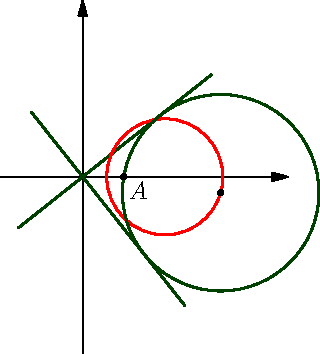
\includegraphics{./Cgp14_1.pdf}
 % Cgp14_1.pdf: 0x0 pixel, 0dpi, nanxnan cm, bb=
 \caption{Exercice \arabic{enumi} Cercles tangents à deux droites}
 \label{fig:Cgp14_1}
\end{figure}

\begin{enumerate}
 \item Le point $I$ est le centre d'un cercle tangent aux deux droites $\mathcal{D}_1$ et $\mathcal{D}_2$ si et seulement si il est à égale distance des deux droites ou encore si et seulement si il est sur une des deux bissectrices des deux droites.
 \item On se donne les deux droites par leurs vecteurs directeurs $\overrightarrow{e}_\theta$ et $\overrightarrow{e}_{\theta +\frac{\pi}{2}}$:
\begin{displaymath}
 \mathcal{D}_1(\theta)= O+\Vect(\overrightarrow{e}_\theta),\hspace{0.3cm}
 \mathcal{D}_2(\theta)= O+\Vect(\overrightarrow{e}_{\theta +\frac{\pi}{2}})
\end{displaymath}
Les centres des cercles passant par $A$ et tangents aux deux droites sont les points $C$ des bissectrices pour lesquels $AC$ est aussi la distance aux bissectrices.\newline
La distance d'un point $M$ à $\mathcal{D}_1(\theta)$ est 
\begin{displaymath}
|\det(\overrightarrow{OM},\overrightarrow{e}_\theta)| 
\end{displaymath}
Les points de la première bissectrice sont de la forme
 \begin{displaymath}
  O+\lambda \overrightarrow{e}_{\theta +\frac{\pi}{4}}
 \end{displaymath}
Soit $C$ un tel point. En notant $\varphi = \theta +\frac{\pi}{4}$, il s'agit d'une définition \emph{polaire} de $C$. La distance à $\mathcal{D}_1(\theta)$ à $C$ est $\frac{|\lambda|}{\sqrt{2}}$. Sa distance à $A$ est
\begin{displaymath}
 \sqrt{(\lambda\cos \varphi -1)^2 + (\lambda\sin(\varphi))^2}
\end{displaymath}
En élevant au carré, la condition assurant que $C$ est le centre d'un cercle vérifiant les conditions s'écrit donc
\begin{displaymath}
 \frac{\lambda^2}{2}=
(\lambda\cos \varphi -1)^2 + (\lambda\sin(\varphi))^2
\end{displaymath}
En développant et simplifiant puis en passant aux coordonnées cartésiennes, on montre que cette condition est équivalente à
\begin{displaymath}
 (x(C)-2)^2 + y(C)^2 = 2
\end{displaymath}
Le point $C$ doit donc être sur le cercle de centre le point de coordonnées $(2,0)$ et de rayon $\sqrt{2}$.\newline
Les points de la deuxième bissectrice sont de la forme
 \begin{displaymath}
  O+\lambda \overrightarrow{e}_{\theta -\frac{\pi}{4}}
 \end{displaymath}
Soit $C$ un tel point. En notant $\varphi = \theta -\frac{\pi}{4}$, il s'agit d'une définition \emph{polaire} de $C$. La suite des calculs est exactement la même exprimée avec $\varphi$. On obtient donc le même cercle, paramétré différement selon qu'il est coupé par l'une ou l'autre des bissectrices.
\end{enumerate}